\documentclass[12pt]{book}

\usepackage{array,epsfig,enumitem}
\usepackage{amsmath}
\usepackage{amsfonts}
\usepackage{amssymb}
\usepackage{amsxtra}
\usepackage{amsthm}
\usepackage{mathrsfs}
\usepackage{color}
\usepackage{eurosym}
\usepackage{times}
%Here I define some theorem styles and shortcut commands for symbols I use often
\theoremstyle{definition}
\newtheorem{defn}{Definition}
\newtheorem{thm}{Theorem}
\newtheorem{cor}{Corollary}
\newtheorem*{rmk}{Remark}
\newtheorem{lem}{Lemma}
\newtheorem*{joke}{Joke}
\newtheorem{ex}{Example}
\newtheorem*{soln}{Solution}
\newtheorem{prop}{Proposition}

\newcommand{\lra}{\longrightarrow}
\newcommand{\ra}{\rightarrow}
\newcommand{\surj}{\twoheadrightarrow}
\newcommand{\graph}{\mathrm{graph}}
\newcommand{\bb}[1]{\mathbb{#1}}
\newcommand{\Z}{\bb{Z}}
\newcommand{\Q}{\bb{Q}}
\newcommand{\R}{\bb{R}}
\newcommand{\C}{\bb{C}}
\newcommand{\N}{\bb{N}}
\newcommand{\M}{\mathbf{M}}
\newcommand{\m}{\mathbf{m}}
\newcommand{\MM}{\mathscr{M}}
\newcommand{\HH}{\mathscr{H}}
\newcommand{\Om}{\Omega}
\newcommand{\Ho}{\in\HH(\Om)}
\newcommand{\bd}{\partial}
\newcommand{\del}{\partial}
\newcommand{\bardel}{\overline\partial}
\newcommand{\textdf}[1]{\textbf{\textsf{#1}}\index{#1}}
\newcommand{\img}{\mathrm{omega}}
\newcommand{\ip}[2]{\left\langle{#1},{#2}\right\rangle}
\newcommand{\inter}[1]{\mathrm{int}{#1}}
\newcommand{\exter}[1]{\mathrm{ext}{#1}}
\newcommand{\cl}[1]{\mathrm{cl}{#1}}
\newcommand{\ds}{\displaystyle}
\newcommand{\vol}{\mathrm{vol}}
\newcommand{\cnt}{\mathrm{ct}}
\newcommand{\osc}{\mathrm{osc}}
\newcommand{\LL}{\mathbf{L}}
\newcommand{\UU}{\mathbf{U}}
\newcommand{\support}{\mathrm{support}}
\newcommand{\AND}{\;\wedge\;}
\newcommand{\OR}{\;\vee\;}
\newcommand{\Oset}{\varnothing}
\newcommand{\st}{\ni}
\newcommand{\wh}{\widehat}

%Pagination stuff.
\setlength{\topmargin}{-.3 in}
\setlength{\oddsidemargin}{0in}
\setlength{\evensidemargin}{0in}
\setlength{\textheight}{9.in}
\setlength{\textwidth}{6.5in}
\pagestyle{empty}

\begin{document}

\begin{center}
{\Large DATA 221 \\  Homework 5  (rev 0)}\\
\textbf{W. Trimble}\\ %You should put your name here
Due: Tuesday 2023-05-02  - 11:59pm
\end{center}

\vspace{0.2 cm}



Kaggle user \texttt{hugodarwood} created a dataset with over 20,000 recipes from the website Epicurious, scraped in 2017:

\texttt{https://www.kaggle.com/datasets/hugodarwood/epirecipes/code}. 

Loosely speaking, there are a few groups of variables in the dataset: nutritional variables (`calories`, `protein`, `fat`, `sodium`),  Ingredient tags (`almond`, `amaretto`, `anchovy`...), Place tags (`alabama`, `alaska`, `aspen`,...), and Other tags (`advance.prep.required`, `anthony.bourdain`, etc.).

You may want to carry out your own exploratory dataset to a) become familiar with the dataset, and b) carry out some pre-processing on the dataset. You will have to make choices during pre-processing--these choices are up to you. We are happy to offer suggestions during office hours, but as long as you feel that you have made a reasonable choice, we will not take points off.   

Once you have pre-processed the data...

\begin{enumerate}

  \item Logistic Regression with $\ell_1$ Regularization
  \begin{enumerate}
    \item Find the logistic regression coefficients to predict whether a recipe has the `pie` tag using $\ell_1$ regularization.  
    \item Plot the regression coefficients as a function of the (logarithm of the) regularization parameter $t$--example on the second page of the assignment. 
    \item Find the optimum regularization parameter $t$ by optimizing for minimum error on a test set.
  \end{enumerate}
  
\item Regression / nutritional information
  \begin{enumerate}
    \item Train a (linear regression?  neural network?)  model to predict the nutrition information fields from everything else.  
    \item  Evaluate your model on a testing holdout set, report its accuracy, and predict the nutrition information for the rows where nutrition information is missing.
    \item  Which coefficents are the largest?  (Salted?  Fried?  protein-feed-enhanced?)
  \end{enumerate}

  \item Principal Component Analysis 
  \begin{enumerate}
    \item Perform Principal Component Analysis (a.k.a., singular value decomposition) on all the features of the dataset. 
    \item Make a graph showing the total fraction of variance in the first N principal components.   How many principal components do you need to retain half of the variance of the data?
    \item Display scatter plots of the first two principal components, PC1 and PC2, for the two response variable classes. Label the axes with the fraction of the variance explained by PC1 and PC2. 
  \end{enumerate}

  \item Embedding 
  \begin{enumerate}
    \item Calculate the all-against all distance matrix in Euclidean space for the category labels.  Produce a clustering.
    \item Calculate the all-against all distance matrix with a Minkowski metric for the category labels.  Produce a clustering.
    \item Map the category labels to a word2vec language embedding, calculate an all-against-all distance matrix, and produce a clustering. 
    \item Plot the three clusterings in principal coordinates space with the conventional (PC 1, 1.2\%...) labels.
  \end{enumerate}

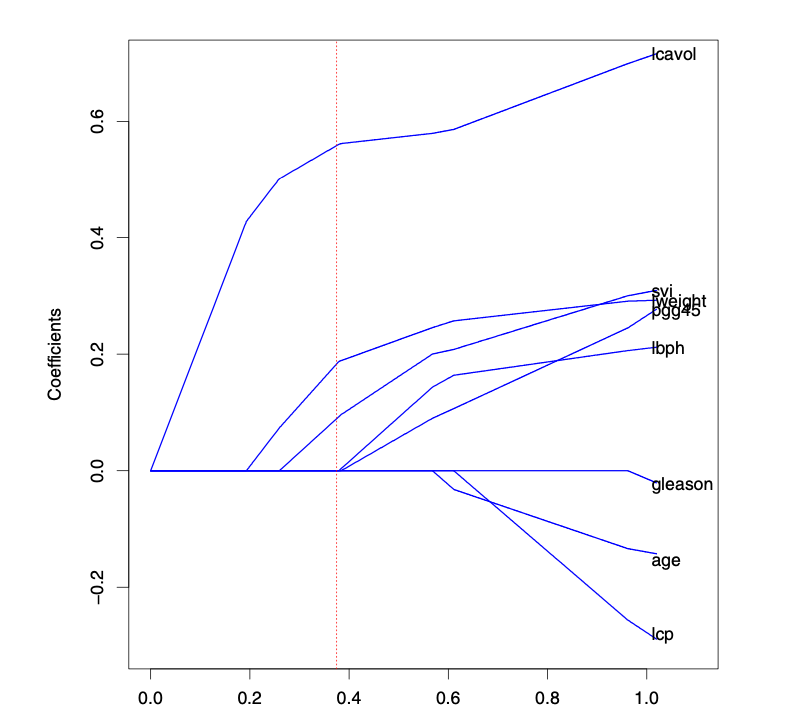
\includegraphics[width=10cm]{images/HASTIE-LASSO.png}


\end{enumerate}
\end{document}


